% Adjust these for the path of the theme and its graphics, relative to this file
%\usepackage{beamerthemeFalmouthGamesAcademy}
\usepackage{../../beamerthemeFalmouthGamesAcademy}
\usepackage{multimedia}
\graphicspath{ {../../} }

% Default language for code listings
\lstset{language=C++,
        morekeywords={each,in,nullptr,int32, TCHAR, uint8, int8, uint16, int16,
        uint32, int32, uint64, int64, PTRINT, UObject. AActor, SWidget, FName,
        FString, UClass, USoundCue, UTexture}
}

% For strikethrough effect
\usepackage[normalem]{ulem}
\usepackage{wasysym}
\usepackage{listings}
\usepackage{pdfpages}

% http://www.texample.net/tikz/examples/state-machine/
\usetikzlibrary{arrows,automata}

\newcommand{\modulecode}{COMP260}\newcommand{\moduletitle}{Distributed Systems}\newcommand{\sessionnumber}{5}

\begin{document}
\title{\sessionnumber: 12}
\subtitle{\modulecode: \moduletitle}

\frame{\titlepage}

\begin{frame}
	\frametitle{Learning outcomes}
	\begin{itemize}
		\item \textbf{Identify} the various parts of the Arduino and their function
		\item \textbf{Explain} the difference between analog and digital
		\item \textbf{Implement} a basic interface using Arduino and openFrameworks
	\end{itemize}
\end{frame}

%TODO: Nice image of arduino
\begin{frame}
  \frametitle{What is an Arduino?}
  \begin{itemize}
    \item Open Source
    \item The Arduino is a small microcontroller board
    \item Basically, a small computer 
    \item Perfect for rapid prototyping physical computing systems
  \end{itemize}
\end{frame}

%TODO: Update with an image of the sensor actuator diagram
\begin{frame}
	\frametitle{Sensors \& Actuators}
	\begin{figure}
		%\href{https://www.youtube.com/watch?v=gvozcv8pS3c}{ 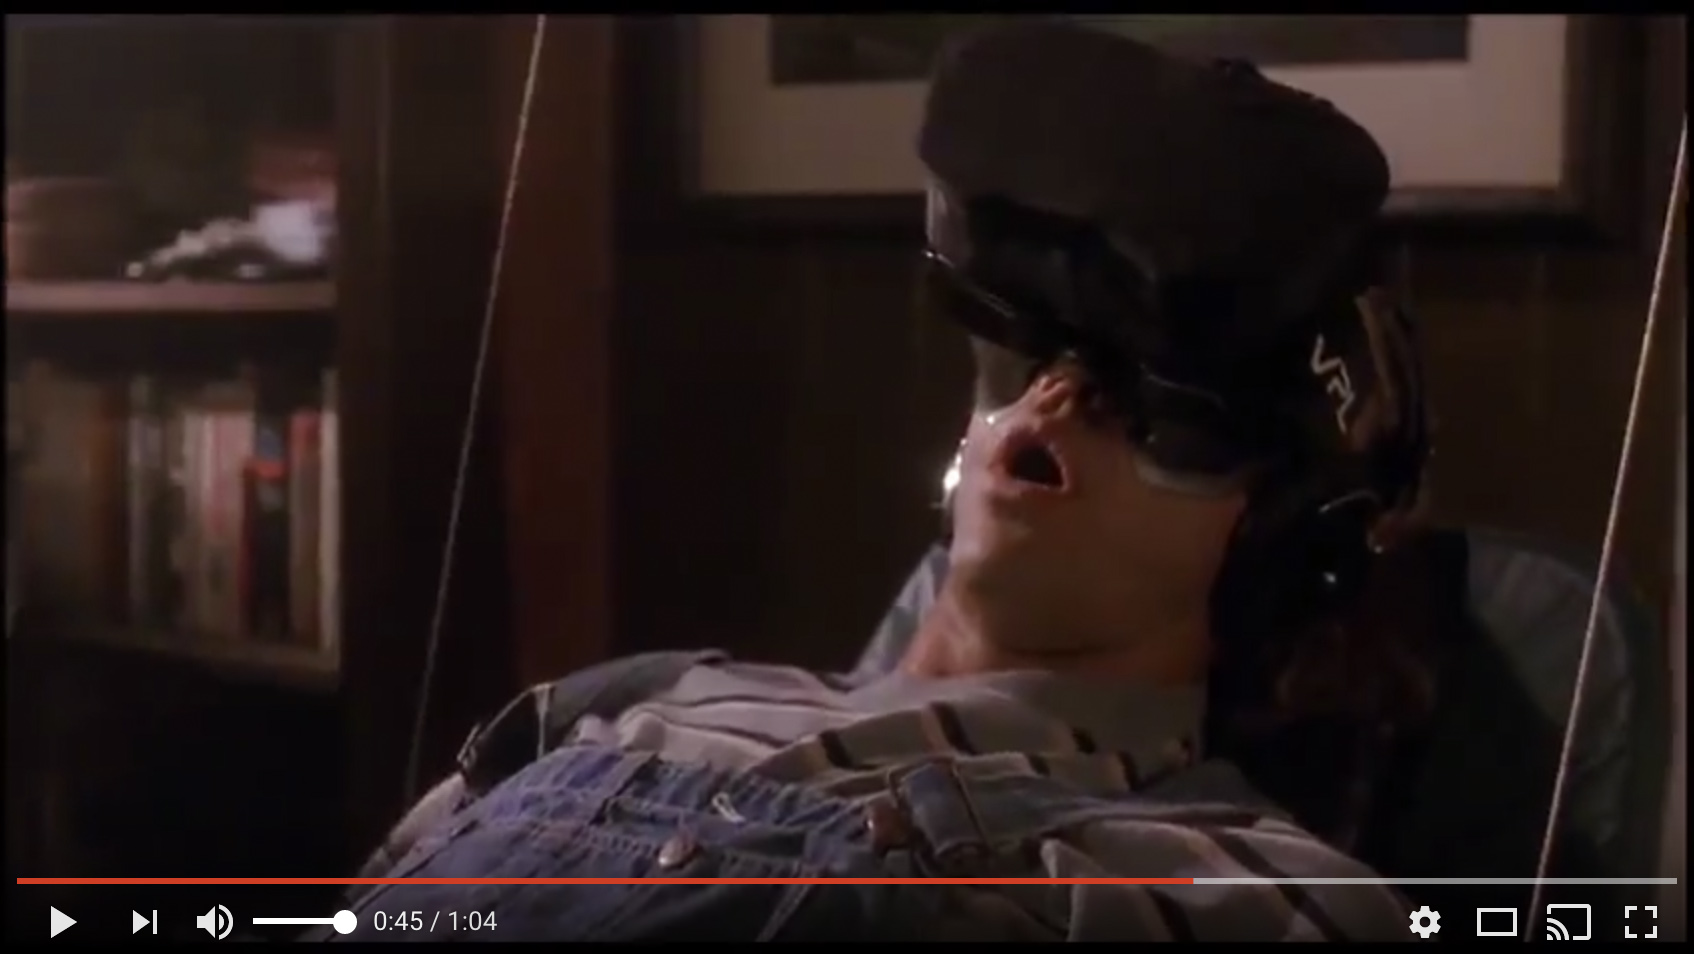
\includegraphics[scale=.3]{assets/mower}  }
		\caption{The Lawn Mower Man - 1992}
	\end{figure}
\end{frame}

\begin{frame}
  \frametitle{The basics}  
  The Arduino can only prcesses electronic signals. This means that stimuli from the physical world need to be transduced to electrical signals before they can be processed from within your code. 
  
  \begin{itemize}
    \item 14 Digital IO pins (0-14)
    \item 6 Analogue in pins(0-5)
    \item 6 Analogue out pins(3,5,6,9,10, and 11) ~
  \end{itemize}
\end{frame}

\begin{frame}
  \frametitle{Power}
	You can power the board using a USB port or DC power supply such as a 9v battery. The Arduino will default to the external power supply if there is one available.   
	%TODO: 9V battery image
\end{frame}

\begin{frame}
	\frametitle{Analogue \& Digital}
\end{frame}

\begin{frame}
  \frametitle{Water Anology}
\end{frame}

\begin{frame}
  \frametitle{Water Anology}
\end{frame}

\begin{frame}
	\frametitle{PWM}
\end{frame}

\begin{frame}
	\frametitle{Serial Communication}
\end{frame}

\begin{frame}
	\frametitle{Driving Bigger Loads}
\end{frame}

\begin{frame}
	\frametitle{Breadboard}
\end{frame}

\begin{frame}
	\frametitle{Shields}
\end{frame}


\end{document}
